\documentclass[12pt,letterpaper,noanswers]{exam}
\usepackage[usenames,dvipsnames,svgnames,table]{xcolor}
\usepackage[margin=0.9in]{geometry}
\renewcommand{\familydefault}{\sfdefault}
\usepackage{multicol}
\pagestyle{head}
\header{AM 111 Class 01}{}{Math in computers, p.\thepage}
\runningheadrule
\headrule
\usepackage{siunitx}
\usepackage{graphicx} % more modern
\usepackage{amsmath} 
\usepackage{amssymb} 
\usepackage{hyperref}
\usepackage{tcolorbox}
\newcommand{\vc}[1]{\underline{#1}}
\begin{document}
 \pdfpageheight 11in 
  \pdfpagewidth 8.5in

\noindent 



\section{Preliminaries}
\begin{itemize}
\itemsep0pt
\item There is a pre-class assignment due before Class 02.
\item There will be a skill check in class during Class 02.  The problem info is below.
\item Problem set 01 will be assigned Friday Sept 2 and is due Friday Sept 9 (content from classes 01 and 02).
\item OH this week: today from 2:30-3:30pm in Pierce 316 (my office).
\end{itemize}

\hrule
\vspace{0.2cm}


\noindent\textbf{Big picture}

Many of the math problems you have studied in the past (finding solutions to equations or systems of equations, approximating data by functions, finding maxima or minima of functions, computing derivatives or integrals, finding solutions to differential equations, approximating functions by other functions) can be tackled using computational methods.  Typically these methods produce approximate solutions to the math problem.

During the semester, we will examine three factors in how approximate these solutions are: (1) the sensitivity of the output of a particular function to small changes in the input, (2) how numbers are represented in computers, and (3) the characteristics of the algorithms being used to compute a solution. 

Today's class focuses on factors (1) and (2).

\vspace{0.2cm}
\hrule
\vspace{0.2cm}

\noindent \textbf{Skill check C01 practice}

Let $f(x) = 
\cos x$.  Find the condition number as a function of $x$.  Use relative error to construct your expression.


\vspace{0.2cm}
\hrule
\vspace{0.2cm}

\noindent \textbf{Skill check solution}

Using Taylor expansion to first order about $x$, $f(x+\Delta x)\approx f(x) + \Delta x \left.\dfrac{df}{dx}\right\vert_x$.

Working with a general $f(x)$:
$\text{cond }\# = \left\vert\dfrac{\hat{y}-y}{y} \right\vert / \left\vert\dfrac{\hat{x}-x}{x} \right\vert \approx \left\vert \dfrac{\Delta xf'(x)}{f(x)} \right\vert / \dfrac{\Delta x}{x} = \left\vert x\dfrac{f'(x)}{f(x)}\right\vert$

For $f(x) = \cos x$, we have

$\text{cond }\# \approx \left\vert x \dfrac{-\sin x}{\cos x} \right\vert  = \vert x\tan x\vert$

\vspace{0.2cm}
\hrule
\vspace{0.2cm}

\noindent \textbf{Teams}

Not assigned: work with students sitting nearby.

\vspace{0.2cm}
\hrule
\vspace{0.2cm}

\section{Well conditioned vs ill conditioned problems}

\noindent \emph{Notes based on work by Thomas Fai, APMTH 111 Spring 2017}

\noindent \textbf{Example: error from approximation}

Evaluate $f(x) = \sqrt{x}$ (find the square root of some number).



Ex: Find $y = \sqrt{\pi}$.   $\sqrt{\pi}\approx \sqrt{3}$.  Note that $\sqrt{4} = 2$ and $\sqrt{1} = 1$.

\noindent Use a linear approximation for $\sqrt{3}$ to find an approximate value, $\hat{y}$ for $\sqrt{\pi}$.
\vspace{1in}

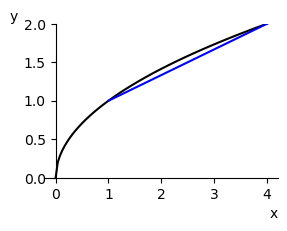
\includegraphics{img/C01linearsqrtapprox.png}



\noindent For $x = \pi$: true solution is $y = 1.77245...$


\noindent The computed solution, $\hat{y}$, would be the true solution with a different input, $\hat{x}$.


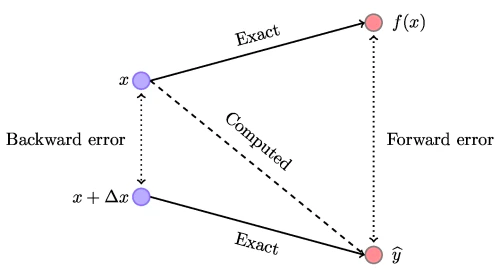
\includegraphics[scale=0.6]{img/C01errorNickHingham.png}

\href{https://nhigham.com/2020/03/25/what-is-backward-error/}{Image from Nick Higham's blog}

\vspace{0.2cm}
\hrule
\vspace{0.2cm}

\noindent \textbf{Definitions: error}

\begin{tcolorbox}
\begin{itemize}
\itemsep0pt
\item The \textbf{forward error} is given by $\left\vert y - \hat{y}\right\vert$ (\textbf{absolute}) or $\left\vert \dfrac{y - \hat{y}}{y}\right\vert$ (\textbf{relative}).
\item The \textbf{backward error} is given by $\left\vert x - \hat{x}\right\vert$ (\textbf{absolute}) or $\left\vert \dfrac{x - \hat{x}}{x}\right\vert$ (\textbf{relative}).
\item The \textbf{condition number} is a measure of the sensitivity of the output to small perturbations in the input \cite{higham2020condition}.  It is given by the ratio of forward to backward error: $\text{cond } \# = \dfrac{\left\vert (y - \hat{y})/y\right\vert}{\left\vert (x - \hat{x})/x\right\vert}$.  

\item If either $x$ or $y$ is close to zero then the condition number may be calculated using absolute error: $\text{cond } \#=\dfrac{\left\vert (y - \hat{y})\right\vert}{\left\vert (x - \hat{x})\right\vert}$
\end{itemize}

\end{tcolorbox}


\vspace{0.2cm}
\hrule
\vspace{0.2cm}

\noindent \textbf{Condition number}

Consider $y = f(x)$ for some function $f$.  If the condition number is $\approx 1$, and you change your input value by $1\%$, how do you expect the output value to change?

\vspace{0.5in}


What if the condition number is $100$?  In this case, if you change your input value by $1\%$, how do you expect the output value to change?

\vspace{0.5in}


\begin{tcolorbox}
\begin{itemize}
\itemsep0pt
\item A problem is \textbf{well conditioned} when small changes in the input lead to comparably small changes in the output.

\item A problem is \textbf{ill conditioned} when the output is sensitive to small changes in the input (or the reverse).
\end{itemize}

\end{tcolorbox}


\noindent \textbf{Condition number examples}

Set $\hat{x} = x+ \Delta x$, so $\Delta x$ is the backward error.  Use linear approximation / Taylor expansion to find the condition number (as a function of $x$) for the following functions.

\emph{Recall: to first order (a linear approximation), $f(\hat{x}) \approx f(x) + (\hat{x} - x)f'(x)$}

\begin{enumerate}
    \item   Let $f(x) = ax + b$.  Find the condition number.
    \vspace{0.5in}
    
    \item Let $f(x) = e^x$.  Find the condition number.
        \vspace{1in}
    
     \item Let $f(x) = \sin x$.  Find the condition number.
         \vspace{1in}

\end{enumerate}

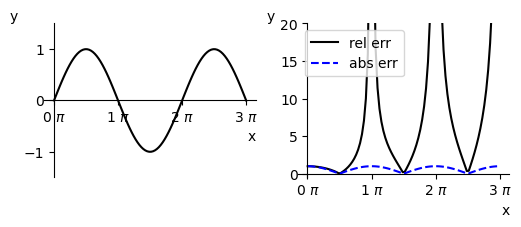
\includegraphics{img/C01sin.png}

\vspace{0.2cm}
\hrule
\vspace{0.2cm}

\noindent \textbf{Sources of error in solving problems computationally}
\begin{tcolorbox}
\begin{enumerate}
\itemsep0pt
    \item The problem is ill-conditioned, so will be sensitive to small changes in the input ($\text{cond }\# \gg 1$ or to small changes in the output ($\text{cond }\# \ll 1$).  This is a feature of the problem itself (not the methods used to tackle the problem).
    \item Instability of the solution method.  A stable algorithm gives exactly the right answer to a nearby problem (i.e. small backward error).
    
\end{enumerate}
\end{tcolorbox}

\section{Representing numbers in a computer (floating point)}

In a computer, we assign finite memory to store each number.  
\begin{itemize}
\itemsep0pt
    \item Only some numbers can be represented: there is no continuity.  Every number has a neighborhood about it with no other numbers.
    \item Numbers for which the representation would be infinite are always shortened (ex: $\pi$, $\sqrt{2}$, $0.\bar{3}$).
\end{itemize}

\begin{tcolorbox}
\begin{itemize}
\itemsep0pt
    \item A \textbf{floating point number} consists of three parts: the \textbf{sign} of the number, the string of bits (\textbf{mantissa}), and an \textbf{exponent}.  \cite{sauer2018numerical}
    \item These parts are stored together.
    \item A floating point system can be characterized by four numbers:
\begin{itemize}
\itemsep0pt
    \item $\beta$ (base)
    \item $p$ (precision)
    \item $[L,U]$ (range for exponents)
\end{itemize}

\item A floating point number is of the form \[ \pm \left(d_0 + d_1\beta^{-1} + d_2 \beta^{-2} + ... + d_{p-1}\beta^{-(p-1)}\right) \beta^E\] where $0\leq d_i\leq \beta-1$ and $L\leq E \leq U$ are integers.

In base $10$ you would write $d_0.d_1d_2...d_{p-1} \times 10^E$.
\item $\pm$ is the sign, $d_0d_1d_2...d_{p-1}$ is the mantissa, $E$ is the exponent, and $p$ is the precision.
\item In a \textbf{normalized} system we require $d_0\neq 0$.
\end{itemize}

\end{tcolorbox}

\noindent\textbf{Example} 

Consider a normalized floating point system with $\beta = 10$, $p = 4$, $-5\leq E \leq 5$.
\begin{itemize}
    \item For numbers in this system, find the smallest number $\epsilon$ such that $1+\epsilon > 1$.  This number is referred to as machine epsilon, $\epsilon_{\text{mach}}$
    \vspace{0.7in}
    
    \item How would you represent $\pi$ in this system?  \emph{If there are multiple options, explain your choice.}
    \vspace{1in}
\end{itemize}


\begin{itemize}
\item Find the smallest number represented in the system.  This is the underflow level (UFL).
\vspace{0.5in}

\item Find the largest number represented in the system.  This is the overflow level (OFL).
\vspace{0.5in}

\item Compute $1.0\times 10^{-5}+ 1$ within this system.
\vspace{0.5in}
\end{itemize}

Note: $1.0\times 10^{-5} + 1.0\times 10^{-5} = 2\times 10^{-5}$ 

but $(\num{1.0e-5} + 1) + (\num{1.0e-5}-1) = 0$.  This is called \textbf{catastrophic cancellation}.

\vspace{0.2cm}
\hrule
\vspace{0.2cm}

\noindent\textbf{Rounding}
\begin{tcolorbox}
\begin{itemize}
\itemsep0pt
    \item Let $\text{fl}(x)$ denote the floating point approximation to $x$.
    \item To convert from $x$ to $\text{fl}(x)$ one option is to \textbf{chop}, taking the first $p$ digits.  
    
    Dropping the $p+1$st digit leads to a relative error of $\left\vert\dfrac{\text{fl}(x) - x}{x}\right\vert\leq \beta^{-(p-1)}$
    \item Another option is \textbf{rounding to nearest} by taking the floating point number nearest to $x$.  
    
    This leads to a relative error of $\left\vert\dfrac{\text{fl}(x) - x}{x}\right\vert\leq \frac{1}{2}\beta^{-(p-1)}$
    
    Note: If $x$ is equidistant between two floating point numbers (think of $1.5$ when rounding to the nearest integer), then the value of $d_{p-1}$ is used to determine whether to round up or down.  
    \item The maximum relative error gives the accuracy of the floating point system.  It is \[\epsilon_{\text{mach}} = \max\limits_{x\in[\text{UFL,OFL}]} \left\vert\dfrac{\text{fl}(x) - x}{x}\right\vert.\]
\end{itemize}
\end{tcolorbox}

\noindent\textbf{Example}.

Let $\beta = 10$, $p =2$.

\begin{tabular}{c|c|c}
     & chop & nearest \\
     \hline
  2.344   & & \\
2.351 & & \\
2.389 & & \\
2.350 & & \\
\end{tabular}


\vspace{0.2cm}
\hrule
\vspace{0.2cm}
\noindent\textbf{Binary}

\begin{tcolorbox}
\begin{itemize}
\itemsep0pt
    \item The floating point systems used in computers typically have $\beta = 2$ (binary), so the digits of the floating point numbers, $d_i = 0$ or $1$.  We will use $b_i$ interchangeably with $d_i$ when we are working in binary.
    \item A single binary digit is called a \textbf{bit}.
    \item In double precision, a floating point number has $64$ bits.  \[s e_1e_2...e_{11}b_1b_2...b_{52}\] where $s$ is the sign, followed by $11$ bits for the exponent, and then the $52$ bits following the decimal point (also called the \textbf{binary point} or \textbf{radix point}).
    \item A few exceptional numbers also need to be represented: NaN (not a number, i.e. 0/0), Inf (infinity, i.e. $1/0$), 0 (note that $d_0 = 1$ so $0$ needs a special representation)
\end{itemize}
\end{tcolorbox}

\vspace{0.2cm}
\hrule
\vspace{0.2cm}

% \noindent\textbf{Converting between binary and decimal}

% One method for decimal integer to binary: 
% \begin{itemize}
% \itemsep0pt
%     \item To read off the digits of $548$, divide by $10$ (shift the decimal place to the left) and keep the remainder.  
    
%     $548/10 = 54.8 = 54$ R$8$ 
    
%     $54/10 = 5.4 = 5$ R$4$
    
%     Reconstruct the number: $548$.
%     \item To find the bits, divide by $2$ (shift the binary place to the left) and keep the remainder.
    
%     $548/2 = 274$ R$0$ 
    
%     $274/2 = 137$ R$0$
    
%     $137/2 = 68$ R$1$
    
%     $68/2 = 34$ R$0$
    
%     $34/2 = 17$ R$0$
    
%     $17/2 = 8$ R$1$
    
%     $8/2 = 4$ R$0$
    
%     $4/2 = 2$ R$0$
    
%     $2/2 = 1$ R$0$
    
%     Now reconstruct: $1000100100 = 2^2+2^5+2^{9} = 4 + 32 + 512 = 548$.
    
% \end{itemize}

% \noindent\textbf{Examples}


% Convert $3$ to binary.
% \vspace{0.5in}

% Convert $700$ to binary.
% \vspace{1in}



\bibliographystyle{plain}
\bibliography{AM111references.bib}


\end{document}